%(BEGIN_QUESTION)
% Copyright 2010, Tony R. Kuphaldt, released under the Creative Commons Attribution License (v 1.0)
% This means you may do almost anything with this work of mine, so long as you give me proper credit

Calculate the amount of voltage dropped across the RTD element in this circuit, the amount of voltage output by the operational amplifier, and the amount of temperature measurement error based on the discrepancy between those two voltages:

$$\includegraphics[width=15.5cm]{i00041x01.eps}$$

$V_{RTD}$ = \underbar{\hskip 50pt}

\vskip 10pt

$V_{out}$ = \underbar{\hskip 50pt}

\vskip 10pt

Temp. error = \underbar{\hskip 50pt}

\vskip 20pt

Note: the RTD in this circuit is a ``100 ohm'' platinum sensor, but its actual resistance at this temperature is 104.2 $\Omega$.

\vfil 

Note: in order to simplify your analysis, you may assume the current through the 1 M$\Omega$ resistors to be zero.  The actual current is so small as to be negligible.

\underbar{file i00041}
\eject
%(END_QUESTION)





%(BEGIN_ANSWER)

This is a graded question -- no answers or hints given!

%(END_ANSWER)





%(BEGIN_NOTES)

You will {\it not} be able to solve for voltages and currents in this circuit by simply applying memorized gain formulae for opamp amplifier circuits, since this is not a regular amplifier circuit.  Instead, you must analyze it based on ``first principles'' (e.g. Kirchhoff's Voltage Law, Ohm's Law, the simplifying assumptions of negative feedback opamp circuits, etc.).

\vskip 10pt

With regard to negative feedback opamp circuits, always apply these simplifying assumptions to make the analysis manageable:

\begin{itemize}
\item{} Negative feedback will force the output voltage to whatever value is necessary to maintain the differential input voltage at zero.
\item{} Input terminals on the opamp draw negligible current.
\end{itemize}

$$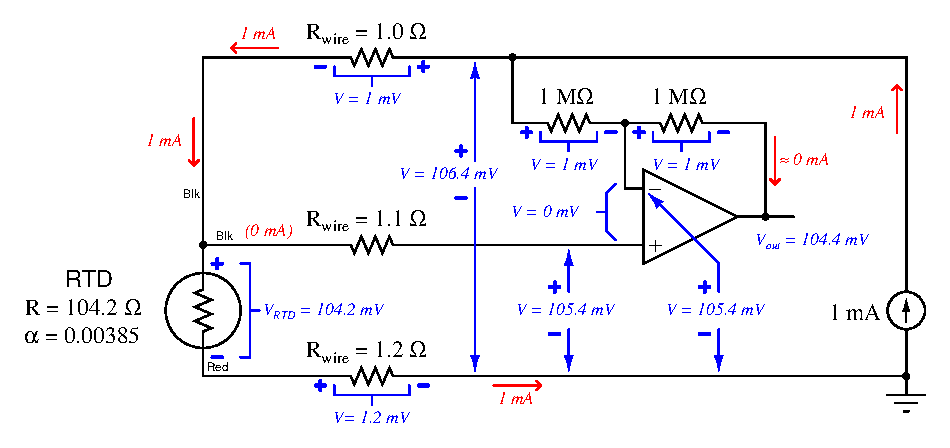
\includegraphics[width=15.5cm]{i00041x02.eps}$$

As you can see here, the RTD drops 104.2 mV while the opamp outputs 104.4 mV, an error of 0.2 mV.  The amount of RTD resistance error equivalent to 0.2 mV (at an excitation current value of 1 mA) is 0.2 ohms.  Given a base resistance of 100 ohms and an alpha coefficient of 0.00385, this resistance error is equivalent to a temperature error of 0.519 $^{o}$C or 0.935 $^{o}$F.


%INDEX% Measurement, temperature: RTD

%(END_NOTES)


